With $\lambda/4$ plate added we can observe the color change when rotating the base of the arrow holder.

\phantom{42}


\begin{minipage}{0.3\textwidth}
    \begin{figure}[h]
    \flushleft
    \vspace{-5mm}
    \animategraphics[loop,controls=play,width=1.0\textwidth]{10}{gifs/g6/}{1}{152} 
    \end{figure}
\end{minipage}
\hfill
\begin{minipage}{0.65\textwidth}
We coud get mean value of rgb color.


It would be interesting to look at RGB in HSV terms. 

\phantom{42}

There are several references to the possibility, in some assumptions to restore wavelength on HSV decomposition.
    \begin{figure}[h]
        \centering
        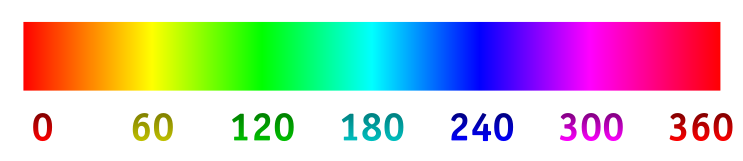
\includegraphics[width=1\textwidth]{figures/HueScale.png}
        % \vspace{-14mm}
        \caption{Hue in the HSV encodings of RGB}
    \end{figure}
\end{minipage}